\chapter{THIẾT KẾ HỆ THỐNG}

\section{Thiết kế luồng nghiệp vụ tổng quát}

Luồng sử dụng chính bắt đầu từ trang giới thiệu. Người dùng chọn đăng nhập, được Auth0 xác thực, sau đó hệ thống tạo hoặc tìm người dùng trong cơ sở dữ liệu. Sau khi vào hệ thống, người dùng có thể cập nhật hồ sơ sức khỏe, xem bài tập, nhận gợi ý, tự lập kế hoạch, theo dõi lịch tập, lưu tiến trình và xem thống kê.


Điểm quan trọng của luồng nghiệp vụ là dữ liệu được truyền qua nhiều bước. Hồ sơ sức khỏe ảnh hưởng đến bài tập gợi ý; bài tập gợi ý có thể được dùng để lập kế hoạch; kế hoạch và bài tập chi tiết tạo ra tiến trình; tiến trình tiếp tục được tổng hợp trong trang thống kê.



\begin{figure}[H]
    \centering
    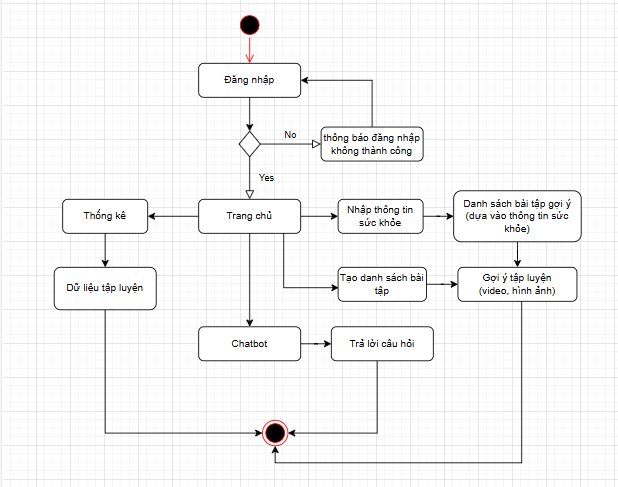
\includegraphics[width=0.86\textwidth,height=0.62\textheight,keepaspectratio]{tai_nguyen/media/image3.png}
    \caption{Luồng sử dụng tổng quan của website}
\end{figure}

\section{Kiến trúc tổng thể của hệ thống}

Hệ thống được chia thành bốn lớp: giao diện người dùng, route xử lý của Remix, cơ sở dữ liệu thông qua Prisma và các dịch vụ ngoài. Giao diện dùng React component và NextUI để tạo màn hình. Route Remix dùng loader để nạp dữ liệu ban đầu và action để xử lý dữ liệu gửi lên. Prisma đảm nhiệm truy vấn cơ sở dữ liệu. Auth0, chatbot và API video là các thành phần tích hợp ngoài.


Kiến trúc này phù hợp với đồ án vì một project có thể quản lý cả frontend và backend. Việc đặt logic trong các route giúp dễ trình bày mối liên hệ giữa màn hình, API và dữ liệu.


\begingroup
\setlength{\tabcolsep}{3pt}
\renewcommand{\arraystretch}{1.25}
\begin{longtable}{|P{0.220\textwidth}|P{0.330\textwidth}|P{0.370\textwidth}|}
\caption{Lớp kiến trúc và thành phần triển khai}\\
\hline
\textbf{Lớp} & \textbf{Thành phần} & \textbf{Vai trò} \\
\hline
\endfirsthead
\caption[]{Lớp kiến trúc và thành phần triển khai (tiếp theo)}\\
\hline
\textbf{Lớp} & \textbf{Thành phần} & \textbf{Vai trò} \\
\hline
\endhead
Giao diện & React, NextUI, Tailwind CSS, Recharts & Hiển thị form, bảng, thẻ bài tập, biểu đồ và chatbot. \\
\hline
Route Remix & loader, action, fetch API & Nạp dữ liệu, xử lý form và kết nối cơ sở dữ liệu. \\
\hline
Dữ liệu & Prisma, PostgreSQL & Lưu người dùng, bài tập, hồ sơ sức khỏe, kế hoạch và tiến trình. \\
\hline
Dịch vụ ngoài & Auth0, Dify/Coze, YouTube API & Xác thực, chatbot và video tham khảo bài tập. \\
\hline
\end{longtable}
\endgroup


\begin{figure}[H]
    \centering
    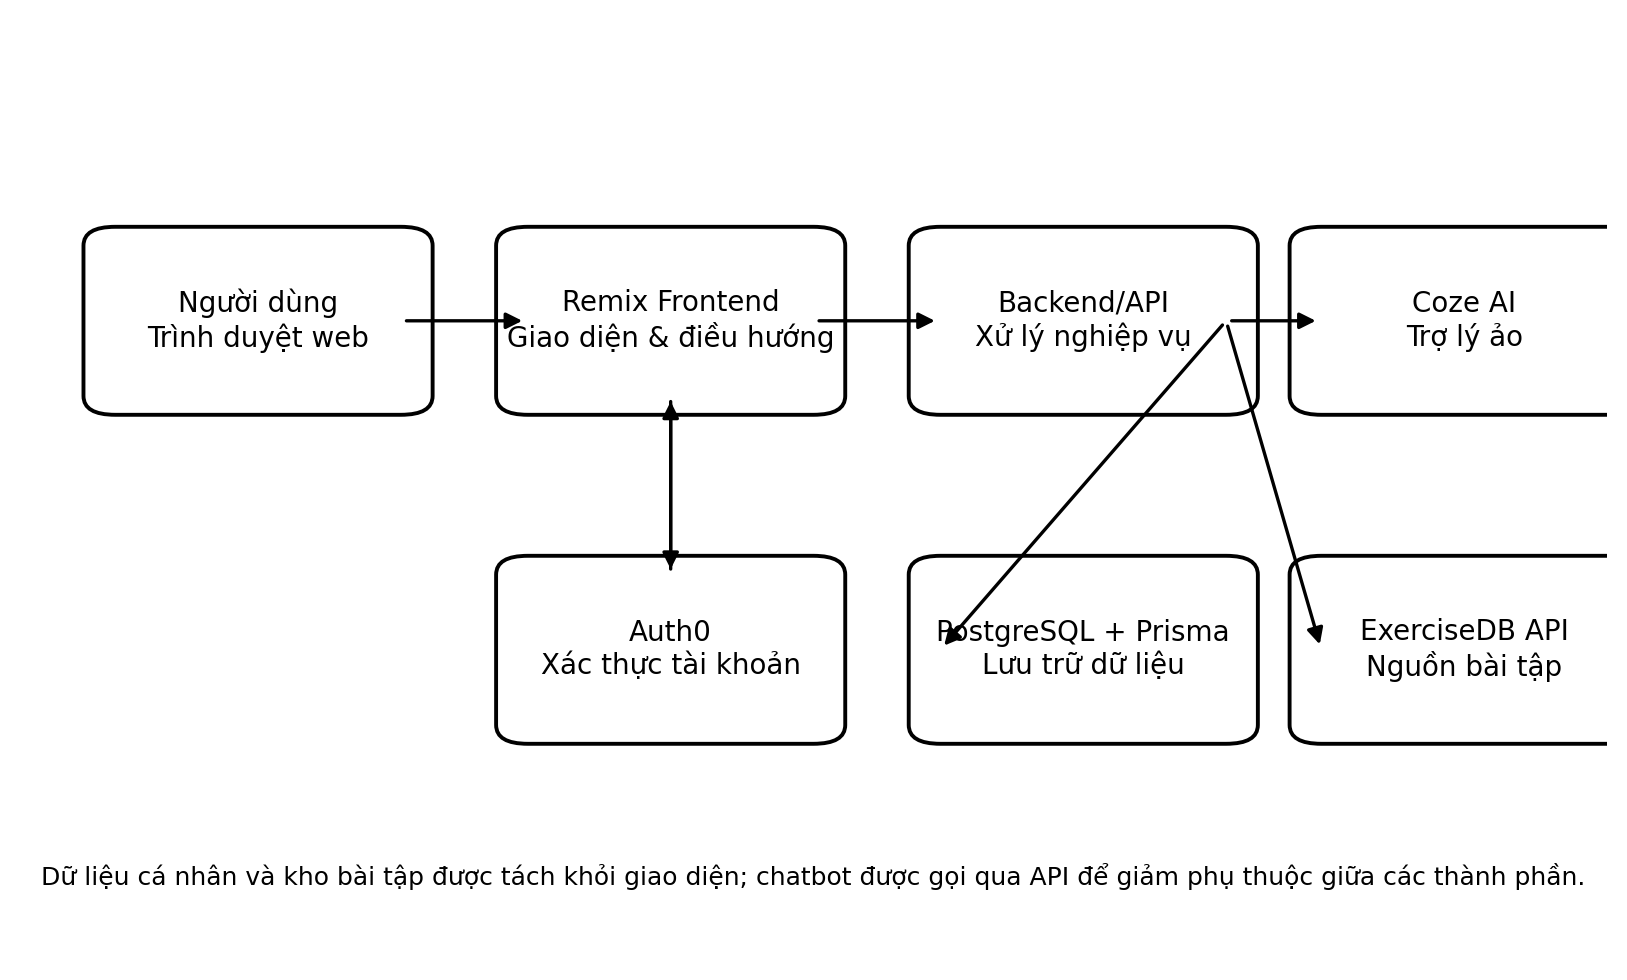
\includegraphics[width=0.86\textwidth,height=0.62\textheight,keepaspectratio]{tai_nguyen/media/image4.png}
    \caption{Kiến trúc logic của website tập luyện}
\end{figure}

\section{Tác nhân và phạm vi quyền}

\begingroup
\setlength{\tabcolsep}{3pt}
\renewcommand{\arraystretch}{1.25}
\begin{longtable}{|P{0.220\textwidth}|P{0.330\textwidth}|P{0.370\textwidth}|}
\caption{Tác nhân và quyền sử dụng}\\
\hline
\textbf{Tác nhân} & \textbf{Quyền chính} & \textbf{Giới hạn} \\
\hline
\endfirsthead
\caption[]{Tác nhân và quyền sử dụng (tiếp theo)}\\
\hline
\textbf{Tác nhân} & \textbf{Quyền chính} & \textbf{Giới hạn} \\
\hline
\endhead
User & Xem bài tập, cập nhật hồ sơ, nhận gợi ý, lập kế hoạch, lưu tiến trình, xem thống kê. & Chỉ thao tác dữ liệu của chính mình. \\
\hline
Admin & Xem dashboard, quản lý người dùng, quản lý bài tập. & Cần tài khoản có cờ isAdmin trong cơ sở dữ liệu. \\
\hline
Auth0 & Xác thực đăng nhập và trả hồ sơ người dùng. & Không xử lý dữ liệu tập luyện. \\
\hline
Chatbot & Trả lời câu hỏi hỗ trợ và hướng dẫn sử dụng. & Không đưa ra kết luận y tế hoặc phác đồ điều trị. \\
\hline
Prisma/Database & Lưu và truy xuất dữ liệu nghiệp vụ. & Không trực tiếp hiển thị giao diện. \\
\hline
\end{longtable}
\endgroup

\section{Đặc tả Use Case tổng quát}

Biểu đồ Use Case tổng quát mô tả mối quan hệ giữa người dùng, quản trị viên và các nhóm chức năng. User tương tác với các chức năng luyện tập, còn Admin chịu trách nhiệm vận hành dữ liệu và theo dõi tổng quan hệ thống.



\begin{figure}[H]
    \centering
    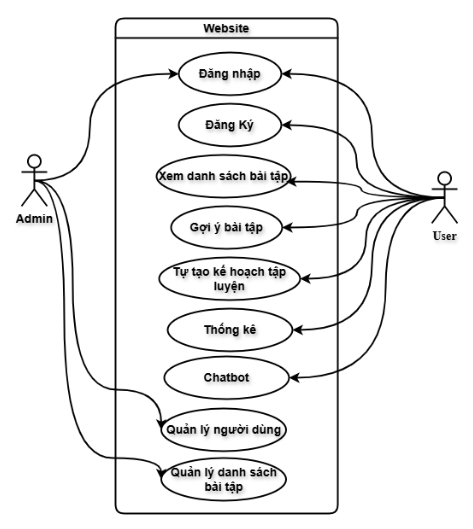
\includegraphics[width=0.86\textwidth,height=0.62\textheight,keepaspectratio]{tai_nguyen/media/image5.png}
    \caption{Use Case tổng thể của hệ thống}
\end{figure}

\begingroup
\setlength{\tabcolsep}{3pt}
\renewcommand{\arraystretch}{1.25}
\begin{longtable}{|P{0.220\textwidth}|P{0.330\textwidth}|P{0.370\textwidth}|}
\caption{Đặc tả Use Case chính}\\
\hline
\textbf{Mã} & \textbf{Tên Use Case} & \textbf{Kết quả mong đợi} \\
\hline
\endfirsthead
\caption[]{Đặc tả Use Case chính (tiếp theo)}\\
\hline
\textbf{Mã} & \textbf{Tên Use Case} & \textbf{Kết quả mong đợi} \\
\hline
\endhead
UC-01 & Đăng nhập & Người dùng được xác thực và chuyển vào hệ thống. \\
\hline
UC-02 & Cập nhật hồ sơ sức khỏe & Thông tin sức khỏe được lưu hoặc cập nhật thành công. \\
\hline
UC-03 & Xem danh sách bài tập & Danh sách bài tập được hiển thị, tìm kiếm và phân trang. \\
\hline
UC-04 & Nhận bài tập đề xuất & Danh sách bài tập phù hợp với hồ sơ được tạo và lưu tạm theo user. \\
\hline
UC-05 & Tạo kế hoạch tập & Các bài tập đã chọn được lưu vào WorkoutPlan. \\
\hline
UC-06 & Lưu tiến trình & Thời gian tập và trạng thái hoàn thành được ghi nhận. \\
\hline
UC-07 & Xem thống kê & Hệ thống tổng hợp dữ liệu 7 ngày, 30 ngày và phản hồi luyện tập. \\
\hline
UC-08 & Quản trị người dùng & Admin xem, sửa hoặc xóa tài khoản. \\
\hline
UC-09 & Quản trị bài tập & Admin thêm, sửa hoặc xóa dữ liệu bài tập. \\
\hline
\end{longtable}
\endgroup

\section{Thiết kế Use Case chi tiết}

Use Case chi tiết được phân rã để làm rõ phạm vi của từng nhóm chức năng. Việc phân rã giúp mỗi chức năng có đầu vào, thao tác và kết quả độc lập, thuận tiện cho kiểm thử về sau.



\begin{figure}[H]
    \centering
    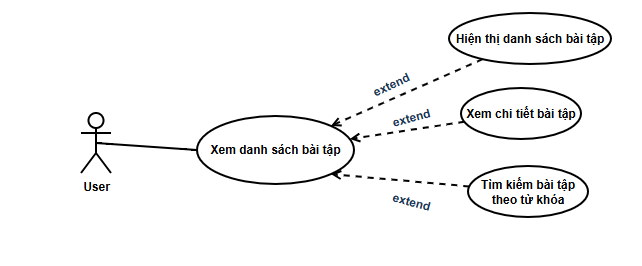
\includegraphics[width=0.86\textwidth,height=0.62\textheight,keepaspectratio]{tai_nguyen/media/image6.png}
    \caption{Use Case chi tiết cho nhóm xem bài tập}
\end{figure}

Use Case chi tiết được phân rã để làm rõ phạm vi của từng nhóm chức năng. Việc phân rã giúp mỗi chức năng có đầu vào, thao tác và kết quả độc lập, thuận tiện cho kiểm thử về sau.



\begin{figure}[H]
    \centering
    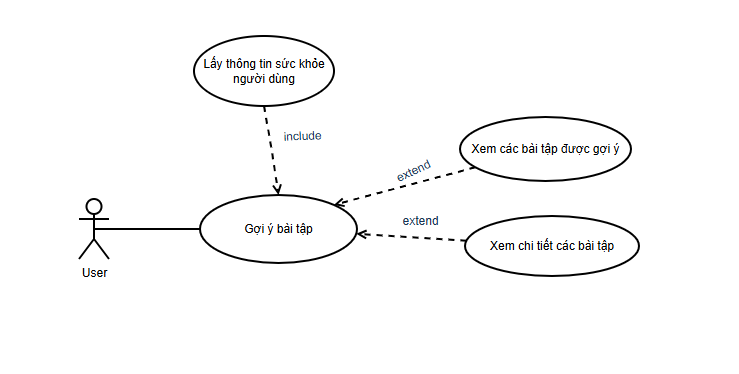
\includegraphics[width=0.86\textwidth,height=0.62\textheight,keepaspectratio]{tai_nguyen/media/image7.png}
    \caption{Use Case chi tiết cho nhóm đề xuất bài tập}
\end{figure}

Use Case chi tiết được phân rã để làm rõ phạm vi của từng nhóm chức năng. Việc phân rã giúp mỗi chức năng có đầu vào, thao tác và kết quả độc lập, thuận tiện cho kiểm thử về sau.



\begin{figure}[H]
    \centering
    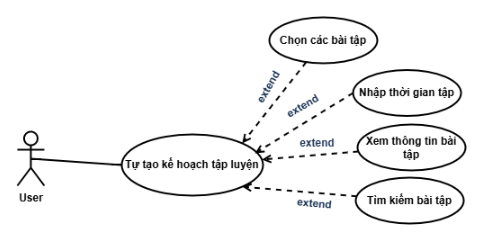
\includegraphics[width=0.86\textwidth,height=0.62\textheight,keepaspectratio]{tai_nguyen/media/image8.png}
    \caption{Use Case chi tiết cho nhóm lập kế hoạch tập}
\end{figure}

Use Case chi tiết được phân rã để làm rõ phạm vi của từng nhóm chức năng. Việc phân rã giúp mỗi chức năng có đầu vào, thao tác và kết quả độc lập, thuận tiện cho kiểm thử về sau.



\begin{figure}[H]
    \centering
    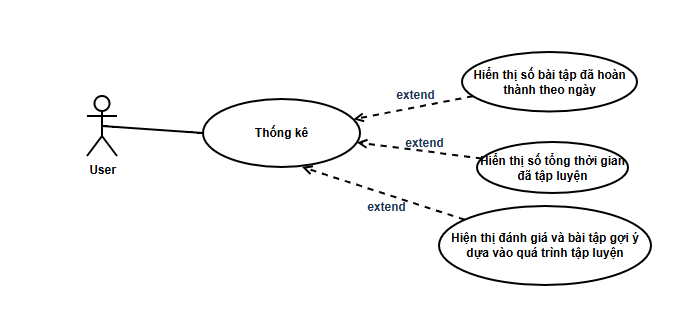
\includegraphics[width=0.86\textwidth,height=0.62\textheight,keepaspectratio]{tai_nguyen/media/image9.png}
    \caption{Use Case chi tiết cho nhóm thống kê tiến trình}
\end{figure}

Use Case chi tiết được phân rã để làm rõ phạm vi của từng nhóm chức năng. Việc phân rã giúp mỗi chức năng có đầu vào, thao tác và kết quả độc lập, thuận tiện cho kiểm thử về sau.



\begin{figure}[H]
    \centering
    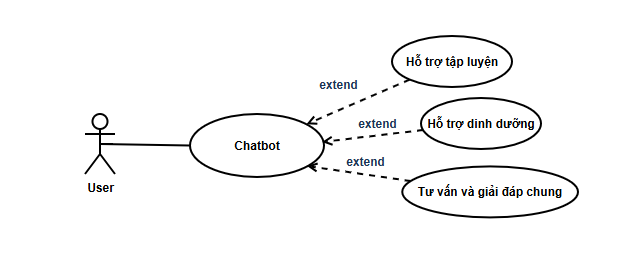
\includegraphics[width=0.86\textwidth,height=0.62\textheight,keepaspectratio]{tai_nguyen/media/image10.png}
    \caption{Use Case chi tiết cho nhóm chatbot}
\end{figure}

Use Case chi tiết được phân rã để làm rõ phạm vi của từng nhóm chức năng. Việc phân rã giúp mỗi chức năng có đầu vào, thao tác và kết quả độc lập, thuận tiện cho kiểm thử về sau.



\begin{figure}[H]
    \centering
    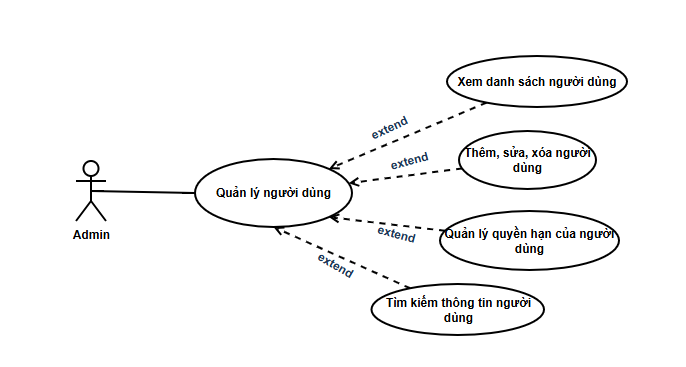
\includegraphics[width=0.86\textwidth,height=0.62\textheight,keepaspectratio]{tai_nguyen/media/image11.png}
    \caption{Use Case chi tiết cho quản trị người dùng}
\end{figure}

Use Case chi tiết được phân rã để làm rõ phạm vi của từng nhóm chức năng. Việc phân rã giúp mỗi chức năng có đầu vào, thao tác và kết quả độc lập, thuận tiện cho kiểm thử về sau.



\begin{figure}[H]
    \centering
    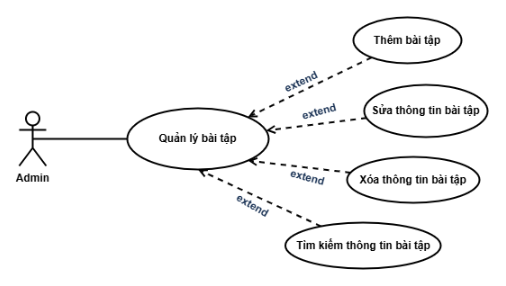
\includegraphics[width=0.86\textwidth,height=0.62\textheight,keepaspectratio]{tai_nguyen/media/image12.png}
    \caption{Use Case chi tiết cho quản trị bài tập}
\end{figure}

\section{Thiết kế chuỗi tương tác xử lý}

Biểu đồ trình tự giúp mô tả thứ tự trao đổi thông tin giữa người dùng, giao diện, route xử lý, cơ sở dữ liệu và dịch vụ ngoài. Các luồng quan trọng gồm đăng nhập, đăng ký, xem bài tập, nhận gợi ý, lưu kế hoạch, thống kê, chatbot và nhóm quản trị.



\begin{figure}[H]
    \centering
    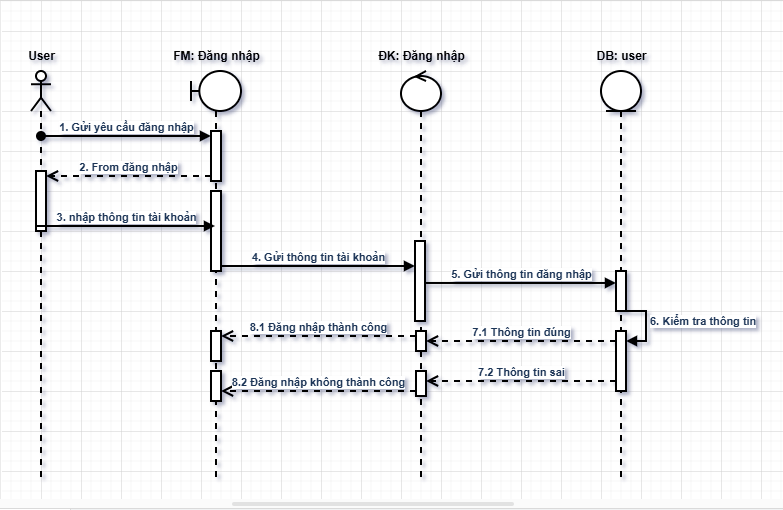
\includegraphics[width=0.86\textwidth,height=0.62\textheight,keepaspectratio]{tai_nguyen/media/image13.png}
    \caption{Trình tự xử lý đăng nhập}
\end{figure}


\begin{figure}[H]
    \centering
    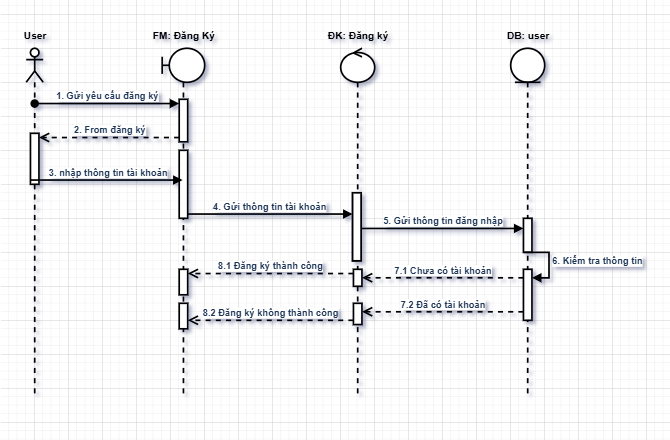
\includegraphics[width=0.86\textwidth,height=0.62\textheight,keepaspectratio]{tai_nguyen/media/image14.png}
    \caption{Trình tự xử lý đăng ký}
\end{figure}


\begin{figure}[H]
    \centering
    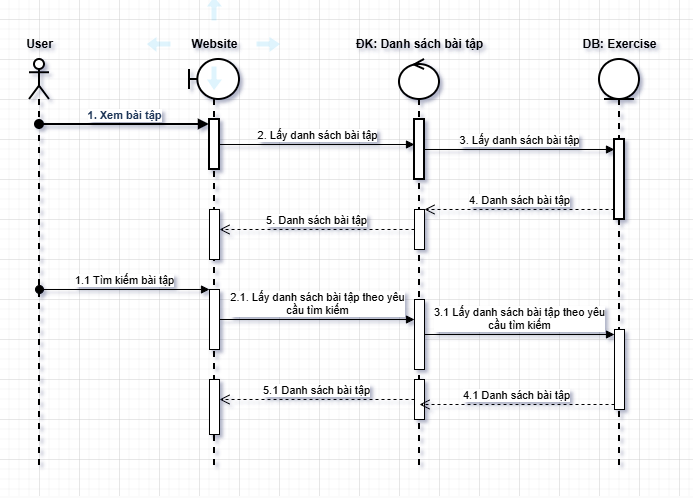
\includegraphics[width=0.86\textwidth,height=0.62\textheight,keepaspectratio]{tai_nguyen/media/image15.png}
    \caption{Trình tự xử lý khi xem thư viện bài tập}
\end{figure}


\begin{figure}[H]
    \centering
    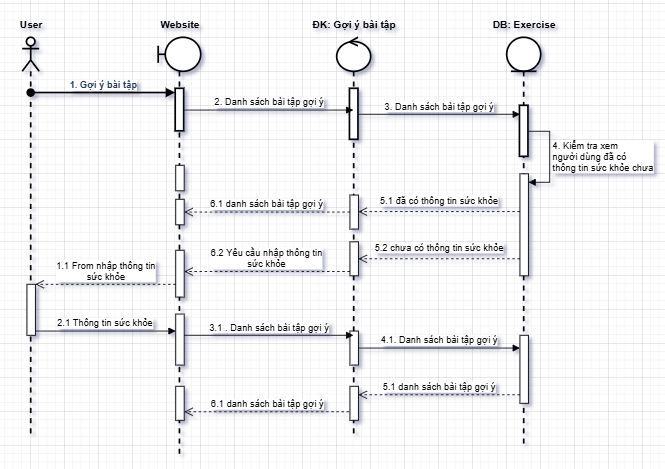
\includegraphics[width=0.86\textwidth,height=0.62\textheight,keepaspectratio]{tai_nguyen/media/image16.png}
    \caption{Trình tự xử lý khi đề xuất bài tập}
\end{figure}


\begin{figure}[H]
    \centering
    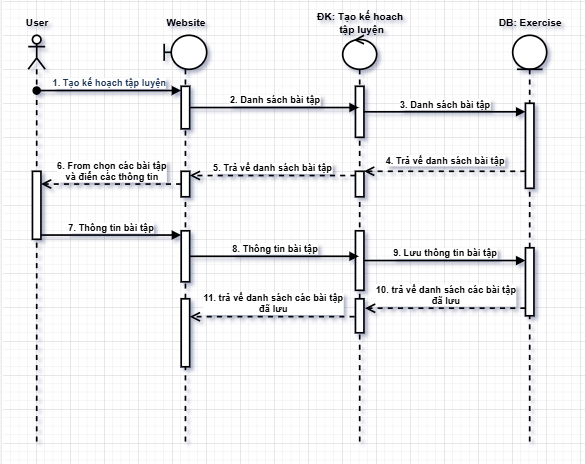
\includegraphics[width=0.86\textwidth,height=0.62\textheight,keepaspectratio]{tai_nguyen/media/image17.png}
    \caption{Trình tự xử lý khi tạo kế hoạch tập}
\end{figure}


\begin{figure}[H]
    \centering
    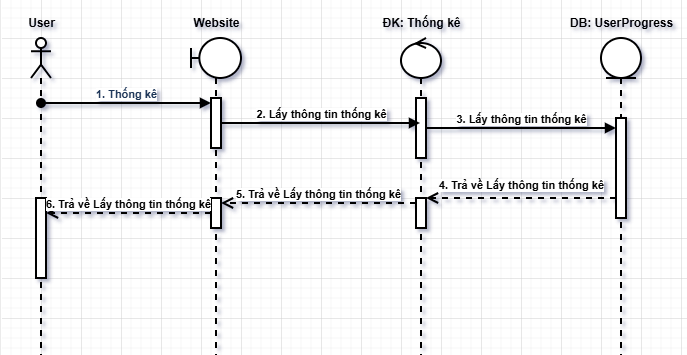
\includegraphics[width=0.86\textwidth,height=0.62\textheight,keepaspectratio]{tai_nguyen/media/image18.png}
    \caption{Trình tự xử lý khi tổng hợp thống kê}
\end{figure}


\begin{figure}[H]
    \centering
    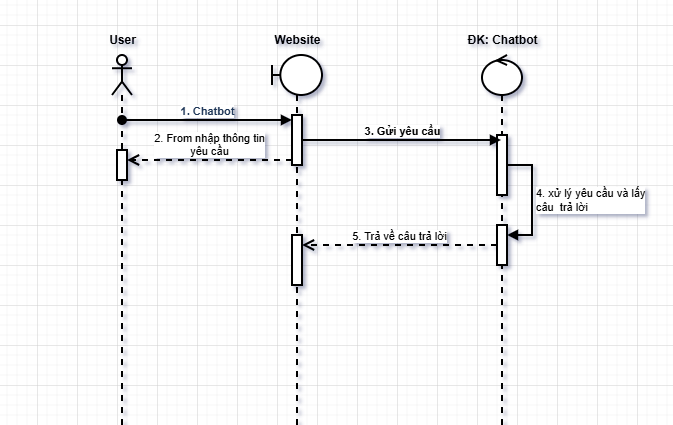
\includegraphics[width=0.86\textwidth,height=0.62\textheight,keepaspectratio]{tai_nguyen/media/image19.png}
    \caption{Trình tự xử lý khi người dùng hỏi chatbot}
\end{figure}


\begin{figure}[H]
    \centering
    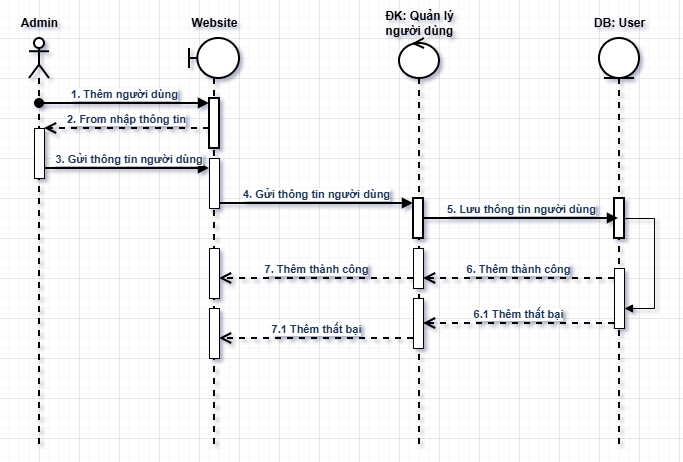
\includegraphics[width=0.86\textwidth,height=0.62\textheight,keepaspectratio]{tai_nguyen/media/image20.png}
    \caption{Trình tự xử lý khi thêm người dùng}
\end{figure}


\begin{figure}[H]
    \centering
    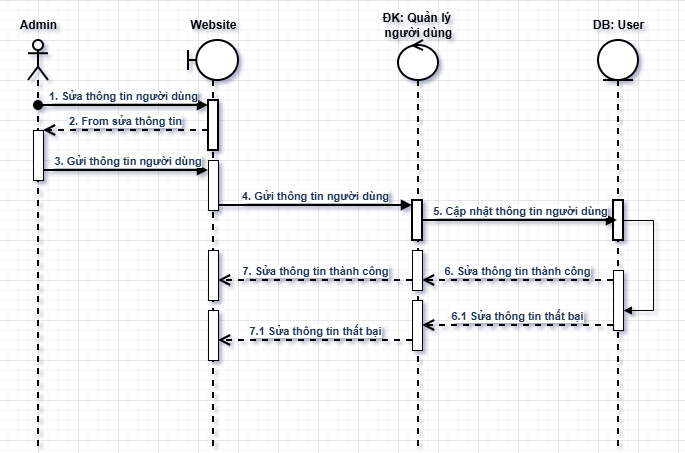
\includegraphics[width=0.86\textwidth,height=0.62\textheight,keepaspectratio]{tai_nguyen/media/image21.png}
    \caption{Trình tự xử lý khi cập nhật người dùng}
\end{figure}


\begin{figure}[H]
    \centering
    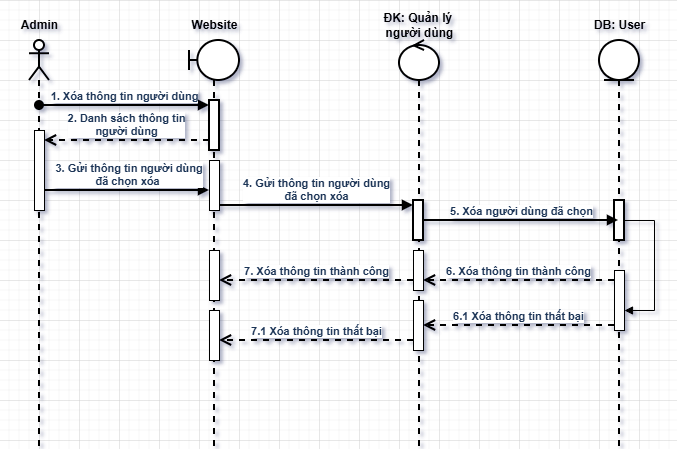
\includegraphics[width=0.86\textwidth,height=0.62\textheight,keepaspectratio]{tai_nguyen/media/image22.png}
    \caption{Trình tự xử lý khi xóa người dùng}
\end{figure}


\begin{figure}[H]
    \centering
    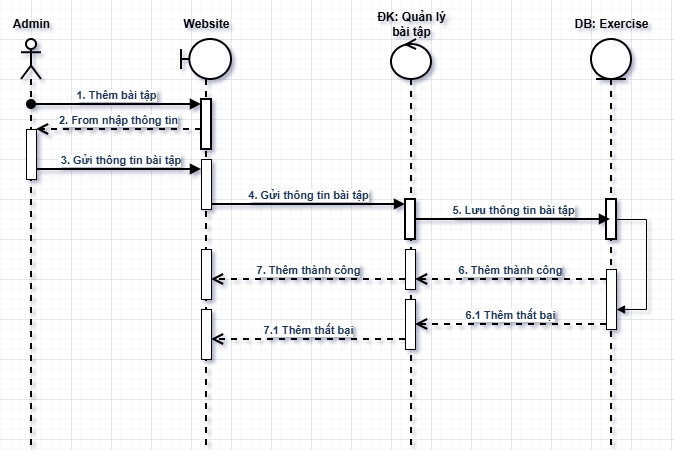
\includegraphics[width=0.86\textwidth,height=0.62\textheight,keepaspectratio]{tai_nguyen/media/image23.png}
    \caption{Trình tự xử lý khi thêm bài tập}
\end{figure}


\begin{figure}[H]
    \centering
    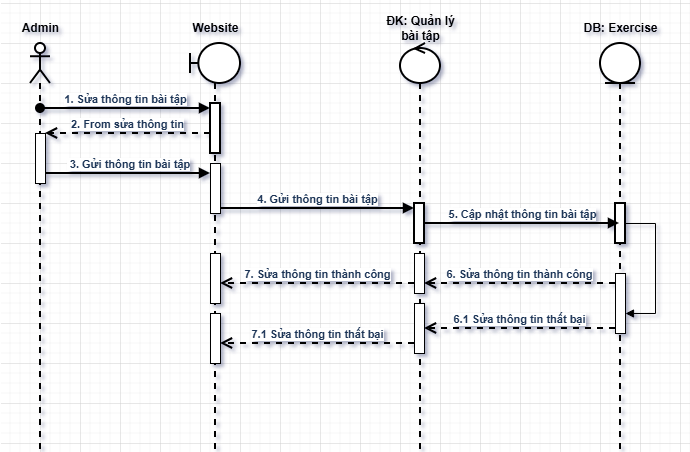
\includegraphics[width=0.86\textwidth,height=0.62\textheight,keepaspectratio]{tai_nguyen/media/image24.png}
    \caption{Trình tự xử lý khi cập nhật bài tập}
\end{figure}


\begin{figure}[H]
    \centering
    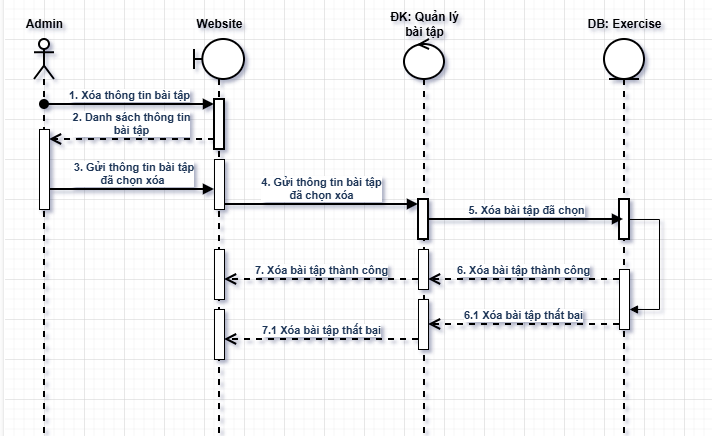
\includegraphics[width=0.86\textwidth,height=0.62\textheight,keepaspectratio]{tai_nguyen/media/image25.png}
    \caption{Trình tự xử lý khi xóa bài tập}
\end{figure}

\section{Thiết kế mô hình dữ liệu}

Mô hình dữ liệu của hệ thống được xây dựng quanh các thực thể chính: User, HealthStatus, Exercise, Workout, WorkoutPlan và UserProgress. User là trung tâm của dữ liệu cá nhân. HealthStatus lưu hồ sơ sức khỏe. Exercise lưu thư viện bài tập. Workout lưu danh sách bài tập đề xuất hoặc bài tập theo người dùng. WorkoutPlan lưu kế hoạch theo ngày. UserProgress ghi nhận tiến trình hoàn thành.


Các quan hệ này giúp hệ thống trả lời được những câu hỏi nghiệp vụ: người dùng hiện có hồ sơ sức khỏe nào, bài tập nào phù hợp, lịch tập đã lưu là gì, bài nào đã hoàn thành và kết quả thống kê trong giai đoạn gần đây ra sao.



\begin{figure}[H]
    \centering
    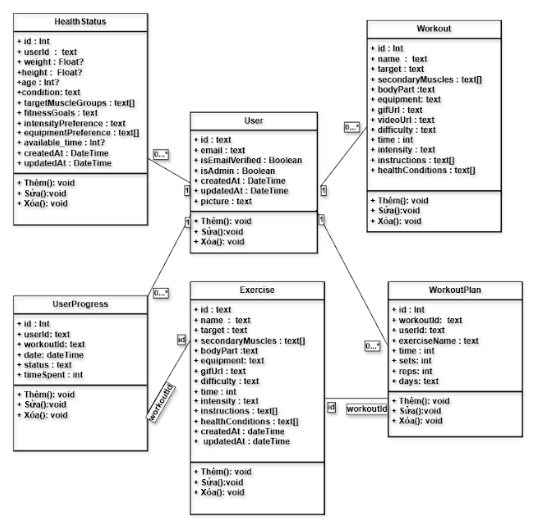
\includegraphics[width=0.86\textwidth,height=0.62\textheight,keepaspectratio]{tai_nguyen/media/image26.png}
    \caption{Mô hình lớp dữ liệu của hệ thống}
\end{figure}

\begingroup
\setlength{\tabcolsep}{3pt}
\renewcommand{\arraystretch}{1.25}
\begin{longtable}{|P{0.220\textwidth}|P{0.330\textwidth}|P{0.370\textwidth}|}
\caption{Mô tả các bảng dữ liệu chính}\\
\hline
\textbf{Bảng/Model} & \textbf{Trường tiêu biểu} & \textbf{Mục đích} \\
\hline
\endfirsthead
\caption[]{Mô tả các bảng dữ liệu chính (tiếp theo)}\\
\hline
\textbf{Bảng/Model} & \textbf{Trường tiêu biểu} & \textbf{Mục đích} \\
\hline
\endhead
User & id, email, userName, picture, isAdmin, isEmailVerified & Quản lý tài khoản và quyền truy cập. \\
\hline
HealthStatus & userId, weight, height, condition, fitnessGoals, intensityPreference & Lưu hồ sơ sức khỏe phục vụ cá nhân hóa. \\
\hline
Exercise & id, name, target, equipment, gifUrl, difficulty, intensity, time & Lưu kho bài tập và thuộc tính lọc. \\
\hline
Workout & userId, exercise fields & Lưu danh sách bài tập được gợi ý cho từng người dùng. \\
\hline
WorkoutPlan & userId, workoutId, date, time, sets, reps & Lưu kế hoạch luyện tập cá nhân. \\
\hline
UserProgress & userId, workoutId, timeSpent, status, date & Ghi nhận tiến trình hoàn thành bài tập. \\
\hline
Message & userId, sender, message & Lưu nội dung hội thoại nếu dùng route chatbotapi. \\
\hline
\end{longtable}
\endgroup

\section{Thiết kế route và API logic}

Trong Remix, route vừa là đường dẫn giao diện vừa có thể là endpoint xử lý dữ liệu. Thiết kế route của hệ thống được chia theo nhóm: xác thực, hồ sơ sức khỏe, bài tập, kế hoạch, tiến trình, thống kê, chatbot và quản trị.


\begingroup
\setlength{\tabcolsep}{3pt}
\renewcommand{\arraystretch}{1.25}
\begin{longtable}{|P{0.220\textwidth}|P{0.330\textwidth}|P{0.370\textwidth}|}
\caption{Ma trận route và chức năng}\\
\hline
\textbf{Route/File} & \textbf{Loại xử lý} & \textbf{Vai trò} \\
\hline
\endfirsthead
\caption[]{Ma trận route và chức năng (tiếp theo)}\\
\hline
\textbf{Route/File} & \textbf{Loại xử lý} & \textbf{Vai trò} \\
\hline
\endhead
auth.auth0.jsx, homeCallback.jsx & loader/action & Điều hướng xác thực Auth0 và nhận callback sau đăng nhập. \\
\hline
login.jsx & loader & Tạo người dùng nếu chưa có và nạp dữ liệu bài tập ban đầu. \\
\hline
home.jsx & loader + giao diện & Hiển thị thư viện bài tập, tìm kiếm và phân trang. \\
\hline
HealthStatus.jsx, healthstatusapi.jsx & loader/action & Nhập, lưu và cập nhật hồ sơ sức khỏe. \\
\hline
equipmentapi.jsx, musclesapi.jsx & loader & Trả danh sách thiết bị và nhóm cơ theo lựa chọn sức khỏe. \\
\hline
Recommended.workout.jsx & loader & Lọc bài tập theo hồ sơ và lưu danh sách gợi ý. \\
\hline
WorkoutPlan.jsx, Workoutplanapi.jsx & loader/action & Chọn bài tập và lưu kế hoạch tập luyện. \\
\hline
Workout.jsx, editworkoutapi.jsx, deleteapi.jsx & loader/action & Xem, sửa và xóa bài tập trong kế hoạch. \\
\hline
ExerciseDetail.jsx, userprogressapi.jsx & loader/action & Xem chi tiết, bật timer và lưu tiến trình. \\
\hline
Stats.jsx & loader + giao diện & Tổng hợp thống kê và phản hồi cá nhân hóa. \\
\hline
admin.jsx & loader + giao diện & Dashboard quản trị, CRUD user và bài tập. \\
\hline
chatbotapi2.jsx & component & Nhúng chatbot vào giao diện website. \\
\hline
\end{longtable}
\endgroup

\section{Thiết kế xử lý bảo mật và phân quyền}

Bảo mật trong hệ thống được triển khai ở nhiều mức. Mức đầu tiên là xác thực qua Auth0. Mức thứ hai là session cookie lưu userId để backend biết người dùng hiện tại. Mức thứ ba là kiểm tra quyền admin trước khi truy cập trang quản trị hoặc thực hiện thao tác quản lý.


Về nguyên tắc, không nên chỉ ẩn nút quản trị ở giao diện. Backend vẫn phải kiểm tra quyền trước khi cho phép sửa hoặc xóa dữ liệu. Điều này đặc biệt quan trọng với các action như update\_user, delete\_user, create\_exercise và delete\_exercise.


Các khóa API, token chatbot, secret session và khóa dịch vụ không nên ghi trực tiếp trong mã nguồn khi triển khai thật. Trong báo cáo, các giá trị cụ thể được lược bỏ hoặc chỉ mô tả vai trò để tránh lộ thông tin nhạy cảm.


\section{Thiết kế giao diện}

Giao diện người dùng được tổ chức theo các màn hình chính: trang giới thiệu, đăng nhập, trang chủ, hồ sơ sức khỏe, bài tập đề xuất, lập kế hoạch, lịch tập, thống kê, chi tiết bài tập và chatbot. Các màn hình dùng navbar và avatar để tạo lối điều hướng thống nhất.


Giao diện quản trị được thiết kế theo tab gồm dashboard, quản lý người dùng và quản lý bài tập. Cách tổ chức này giúp admin không bị lẫn giữa dữ liệu người dùng cuối và dữ liệu bài tập.


\section{Thiết kế thông báo và xử lý lỗi}

Hệ thống cần phản hồi rõ khi người dùng nhập thiếu dữ liệu, chưa có hồ sơ sức khỏe, chưa đăng nhập hoặc thao tác lưu thất bại. Trong mã nguồn, các route thường trả json kèm status 400, 401, 404 hoặc 500 tùy lỗi. Giao diện sử dụng toast để thông báo kết quả thao tác.


Đối với dữ liệu luyện tập, các trường như timeSpent, workoutId, status, sets và reps cần kiểm tra trước khi lưu. Với userprogressapi, nếu thiếu userId, workoutId hoặc timeSpent không hợp lệ, hệ thống trả lỗi thay vì ghi dữ liệu sai vào cơ sở dữ liệu.

